\documentclass[10pt, xcolor={x11names,table},compress]{beamer}
\usepackage{anyfontsize}
%%% Author and Title Information %%%
\newcommand{\titleinfo}{Tidy Finance in Practice:\\ How Explicit Assumptions Avoid Bad Investment Strategies}
\title{\titleinfo}
\def\authora{Christoph Frey}
\def\affa{Lancaster University}
\def\linka{}
\newcommand{\authorinfo}{\authora}
%%% General %%%
\usepackage[english]{babel}
\usepackage[T1]{fontenc}
\usepackage[utf8]{inputenc}
%%% Graphics %%%
\usepackage{color}
\usepackage{graphicx, svg}
\usepackage{tikz}
\usetikzlibrary{shapes,arrows,trees,backgrounds}
%%% Tables %%%
\usepackage{booktabs}
\usepackage{multirow}
\usepackage{array}
\usepackage{tabularx}
%%% Math %%%
\usepackage{bm}
\usepackage{amsmath,amsfonts,amssymb}
%\usepackage{ulem} % double underline with \uuline{}
\usepackage{listings}
\definecolor{codebg}{HTML}{F5F8FA}          % very light teal tint
\definecolor{codeframe}{HTML}{B8D4DC}       % muted teal border
\definecolor{codekw}{HTML}{3B9AB2}          % deep teal — keywords
\definecolor{codecomment}{HTML}{78B7C5}     % light blue — comments
\definecolor{codestring}{HTML}{E1AF00}      % amber — strings
\definecolor{codebuiltin}{HTML}{F21A00}     % red — builtins
\lstset{
  language=Python,
  basicstyle=\ttfamily\small,
  keywordstyle=\color{codekw}\bfseries,
  commentstyle=\color{codecomment}\itshape,
  stringstyle=\color{codestring},
  emphstyle=\color{codebuiltin},
  emph={self,True,False,None,np,pd,lambda},
  backgroundcolor=\color{codebg},
  frame=single,
  framesep=4pt,
  rulecolor=\color{codeframe},
  xleftmargin=6pt,
  xrightmargin=6pt,
  aboveskip=0.8em,
  belowskip=0.4em,
  showstringspaces=false,
  breaklines=true,
  tabsize=4,
  columns=flexible,
  morekeywords={class,def,if,for,import,from,return,lambda,range},
}
%%% Bibliography and Refs %%%
\usepackage{hyperref}
\usepackage{nameref}
\usepackage[labelformat=empty]{caption}
\usepackage[sectionbib]{natbib}
\let\natbibcitet\citet
\renewcommand\citet{\bibpunct{(}{)}{,}{a}{,}{,}\natbibcitet}
\let\natbibcitep\citep
\renewcommand\citep{\bibpunct{(}{)}{;}{a}{,}{;}\natbibcitep}
\setcounter{section}{-1}
\newcommand{\am}[1]{\underset{#1}{\text{argmin} } \,}
% arg min über {}
\newcommand{\amx}[1]{\underset{#1}{\text{argmax}} \,}
% arg max über {}
%\newcommand{\N}[2]{\mathcal{N} \left( \, #1 \, , \, #2 \, \right)}
\newcommand{\IG}[2]{\text{IG} \left( \, #1 \, , \, #2 \, \right)}
\usepackage{subfigure}
%%%%%%%%%%%%%%%%%%%%%%%%%%%%%%%%%%%%%%%%%%%%%%%%%%%%%%%%%%%%%%%%%%%%%%%%%%%%%%%%%%%%%%%%%%%%%
%%% Default Theme
\usetheme{default}
%%% Font Family
\usepackage{cmbright}
%%% Symbol Packages
\usepackage{pifont,stmaryrd,amssymb}
%%% No Navigation Bar
\setbeamertemplate{navigation symbols}{}
%%%%%%%%%%%%%%%%%%%%%%%%%%%
%%%       Colors        %%%
%%%%%%%%%%%%%%%%%%%%%%%%%%%
%%% Wes Anderson — Zissou1 palette
%%% #3B9AB2  #78B7C5  #EBCC2A  #E1AF00  #F21A00
\definecolor{dblue}{HTML}{3B9AB2}   % deep teal — primary
\definecolor{dlblue}{HTML}{78B7C5}  % light blue — secondary
\definecolor{dyellow}{HTML}{EBCC2A} % yellow — accent
\definecolor{dgreen}{HTML}{E1AF00}  % amber — positive / highlight
\definecolor{dred}{HTML}{F21A00}    % red — warning
\setbeamercolor{frametitle}{fg=dblue}
\setbeamertemplate{section in head/foot}{\textcolor{dblue}{\hfill\insertsectionhead}}
\setbeamertemplate{section in head/foot shaded}{\textcolor{black!15}{\hfill\insertsectionhead}}
\hypersetup{colorlinks=true,
	citecolor = dblue,
	%pdfpagelabels=TRUE,
	pdfstartview = {FitH},
	linkcolor = dblue,
	urlcolor  = dblue
}
\setbeamercolor{button}{bg=dblue,fg=white}
%%%%%%%%%%%%%%%%%%%%%%%%%%%
%%%     Title Page      %%%
%%%%%%%%%%%%%%%%%%%%%%%%%%%
\setbeamertemplate{title page}{%
	\vspace*{1cm}
	\Large\structure{{\color{dblue}{{\inserttitle}}}}
	\vskip1em\par
	\normalsize\authora\vskip0.1em\par
	\footnotesize\affa
    %\vskip1.5em\par
	\vspace{1em}
    \vfill
    \raggedright % make following content left-aligned
    \hfill\includesvg[width=0.5\linewidth]{./assets/tidy}
    \vspace{2em}\\
}
%%%%%%%%%%%%%%%%%%%%%%%%%%%
%%%   Headline Set-up   %%%
%%%%%%%%%%%%%%%%%%%%%%%%%%%
\setbeamerfont{headline}{size=\fontsize{6}{6},shape=\scshape} %,family={\fontfamily{phv}}}
\setbeamertemplate{headline}{
	\vspace{0.015\paperheight}
	{\leavevmode
		\begin{beamercolorbox}{section in head/foot}
			\insertsectionnavigationhorizontal{\paperwidth}{\hspace*{0.3ex}}{\hspace*{0.3ex}}
		\end{beamercolorbox}%
		\vspace{0.005\paperheight}}
	\begin{beamercolorbox}[center]{}
		\hspace{0.025\paperwidth}\rule{0.95\paperwidth}{0.5pt}\hspace{0.025\paperwidth}
	\end{beamercolorbox}%
}
%%%%%%%%%%%%%%%%%%%%%%%%%%%
%%%   Footline Set-up   %%%
%%%%%%%%%%%%%%%%%%%%%%%%%%%
\setbeamerfont{footline}{size=\fontsize{6}{6},shape=\scshape}
\setbeamertemplate{footline}{
	\begin{beamercolorbox}[center]{}
		\hspace{0.025\paperwidth}\rule{0.95\paperwidth}{0.5pt}\hspace{0.025\paperwidth}
	\end{beamercolorbox}%
	\leavevmode
	\begin{beamercolorbox}[wd=.5\paperwidth,ht=3.1ex,left]{}
		\hspace*{0.025\paperwidth}\textcolor{dblue}{\insertshorttitle}
	\end{beamercolorbox}%
	\begin{beamercolorbox}[wd=.5\paperwidth,ht=3.1ex,right]{}
		\insertframenumber{} $|$ \inserttotalframenumber \hspace{0.025\paperwidth}
	\end{beamercolorbox}%
	\vspace{0.02\paperheight}
}
%%%%%%%%%%%%%%%%%%%%%%%%%%%
%%%        Blocks       %%%
%%%%%%%%%%%%%%%%%%%%%%%%%%%
\usepackage{tcolorbox}
\tcbuselibrary{theorems}
% Theorem (blue)
\newtcbtheorem[]{theo}{Theorem}{colback=dblue!2,colframe=dblue!30!black,coltitle=dblue,colbacktitle=dblue!10!white,before=\begin{center},after=\end{center},width=0.9\textwidth,left=3pt,right=3pt,toptitle=3pt,bottomtitle=3pt,boxrule=0.2mm,fonttitle=\bfseries}{th}
\newtcbtheorem[]{col}{Corollary}{colback=dblue!2,colframe=dblue!30!black,coltitle=dblue,colbacktitle=dblue!10!white,before=\begin{center},after=\end{center},width=0.9\textwidth,left=3pt,right=3pt,toptitle=3pt,bottomtitle=3pt,boxrule=0.2mm,fonttitle=\bfseries}{th}
% Definition (blue)
\newtcbtheorem[]{defi}{Definition}{colback=dblue!2,colframe=dblue!30!black,coltitle=dblue,colbacktitle=dblue!10!white,before=\begin{center},after=\end{center},width=0.9\textwidth,left=3pt,right=3pt,toptitle=3pt,bottomtitle=3pt,boxrule=0.2mm,fonttitle=\bfseries}{th}
% Lemma (blue)
\newtcbtheorem[]{lem}{Lemma}{colback=dblue!2,colframe=dblue!60!black,coltitle=dblue,colbacktitle=dblue!10!white,before=\begin{center},after=\end{center},width=0.9\textwidth,left=3pt,right=3pt,toptitle=3pt,bottomtitle=3pt,boxrule=0.2mm,fonttitle=\bfseries}{th}
% Proposition (green)
\newtcbtheorem[]{prop}{Proposition}{colback=dgreen!2,colframe=dgreen!60!black,coltitle=dgreen,colbacktitle=dgreen!10!white,before=\begin{center},after=\end{center},width=0.9\textwidth,left=3pt,right=3pt,toptitle=3pt,bottomtitle=3pt,boxrule=0.2mm,fonttitle=\bfseries}{th}
% Proof (green)
\newtcbtheorem[]{prf}{Proof}{colback=dgreen!2,colframe=dgreen!60!black,coltitle=dgreen,colbacktitle=dgreen!10!white,before=\begin{center},after=\end{center},width=0.9\textwidth,left=3pt,right=3pt,toptitle=3pt,bottomtitle=3pt,boxrule=0.2mm,fonttitle=\bfseries}{th}
% Blue Box
\newtcolorbox{bbox}[2][]{colback=dblue!2,colframe=dblue!30!black,coltitle=dblue,colbacktitle=dblue!10!white,before=\begin{center},after=\end{center},width=0.9\textwidth,left=3pt,right=3pt,toptitle=3pt,bottomtitle=3pt,boxrule=0.2mm,fonttitle=\bfseries,title={#2},#1}
% Red Box
\newtcolorbox{rbox}[2][]{colback=dred!2,colframe=dred!30!black,coltitle=dred,colbacktitle=dred!10!white,before=\begin{center},after=\end{center},width=0.9\textwidth,left=3pt,right=3pt,toptitle=3pt,bottomtitle=3pt,boxrule=0.2mm,fonttitle=\bfseries,title={#2},#1}
% Green Box
\newtcolorbox{gbox}[2][]{colback=dgreen!2,colframe=dgreen!30!black,coltitle=dgreen,colbacktitle=dgreen!10!white,before=\begin{center},after=\end{center},width=0.9\textwidth,left=3pt,right=3pt,toptitle=3pt,bottomtitle=3pt,boxrule=0.2mm,fonttitle=\bfseries,title={#2},#1}
%%%%%%%%%%%%%%%%%%%%%%%%%%%
%%% Itemize / Enumerate %%%
%%%%%%%%%%%%%%%%%%%%%%%%%%%
\setbeamertemplate{itemize items}{\fontsize{6}{6}{\raisebox{1.5pt}{\textcolor{dblue}{$\blacktriangleright$}}}}
%\setbeamertemplate{itemize items}{\fontsize{6}{6}{\raisebox{1.5pt}{\textcolor{dblue}{\ding{110}}}}}
\setbeamertemplate{itemize subitem}{\fontsize{5}{5}{\raisebox{1.5pt}{\textcolor{dblue}{\ding{110}}}}}
\setbeamertemplate{itemize subsubitem}{\fontsize{4}{4}{\raisebox{1.5pt}{\textcolor{dblue}{$\triangleright$}}}}
\setbeamertemplate{enumerate item}{%
	\usebeamercolor[dblue]{item projected}%
	%\raisebox{0.5pt}{\scriptsize\insertenumlabel.}%
}
\setbeamertemplate{enumerate subitem}{%
	\usebeamercolor[dred]{item projected}%
	%\raisebox{0.5pt}{\hspace{1em}\scriptsize\insertenumlabel.\insertsubenumlabel}%
}
\setlength{\leftmargini}{1.5em}
\setlength{\leftmarginii}{1.5em}
\setlength{\leftmarginiii}{2em}
\setlength{\labelsep}{0.5em}
%%%%%%%%%%%%%%%%%%%%%%%%%%%
%%%     New Commands    %%%
%%%%%%%%%%%%%%%%%%%%%%%%%%%
% Text Color
\newcommand{\btext}{\textcolor{dblue}}
\newcommand{\btextb}[1]{ \textcolor{dblue}{\textbf{#1}}}
\newcommand{\rtext}{\textcolor{dred}}
\newcommand{\rtextb}[1]{ \textcolor{dred}{\textbf{#1}}}
\newcommand{\gtext}{\textcolor{dgreen}}
\newcommand{\gtextb}[1]{ \textcolor{dgreen}{\textbf{#1}}}
\newcommand{\rrtext}{\textcolor{red}}
\newcommand{\rtextbb}[1]{ \textcolor{red}{\textbf{#1}}}
% Enumerate Counter
\newcounter{saveenumi}
\newcommand{\seti}{\setcounter{saveenumi}{\value{enumi}}}
\newcommand{\conti}{\setcounter{enumi}{\value{saveenumi}}}
% New Envirmoments
%\newcommand{\argmin}{\arg\!\min}
%\newcommand{\argmax}{\arg\!\max}
\newcommand{\N}[2]{\text{N} \left( \, #1 \, , \, #2 \, \right)}
\DeclareMathOperator*{\argmax}{arg\,max\,}
\DeclareMathOperator*{\argmin}{arg\,min\,}
\DeclareMathOperator{\tr}{tr}
\DeclareMathOperator{\diag}{diag}
\newcommand{\balpha}{\mbox{\boldmath$\alpha$}}
\newcommand{\bbeta}{\mbox{\boldmath$\beta$}}
\newcommand{\bmu}{\mbox{\boldmath$\mu$}}
\newcommand{\biota}{\mbox{\boldmath$\iota$}}
\newcommand{\bomega}{\mbox{\boldmath$\omega$}}
\newcommand{\bOmega}{\mbox{\boldmath$\Omega$}}
\newcommand{\bsigma}{\mbox{\boldmath$\sigma$}}
\newcommand{\bSigma}{\mbox{\boldmath$\Sigma$}}
\newcommand{\bgamma}{\mbox{\boldmath$\gamma$}}
\newcommand{\btheta}{\mbox{\boldmath$\theta$}}
\newcommand{\bGamma}{\mbox{\boldmath$\Gamma$}}
\newcommand{\bphi}{\mbox{\boldmath$\phi$}}
\newcommand{\bdelta}{\mbox{\boldmath$\delta$}}
\newcommand{\bPhi}{\mbox{\boldmath$\Phi$}}
\newcommand{\bEta}{\mbox{\boldmath$\eta$}}
\newcommand{\bxi}{\mbox{\boldmath$\xi$}}
\newcommand{\bvarepsilon}{\mbox{\boldmath$\varepsilon$}}
\newcommand{\bepsilon}{\mbox{\boldmath$\epsilon$}}
%%% Beamer-safe wrapper for paper tables %%%
%%% Neutralizes \cellcolor, table float, \caption; forces compact font
\newcommand{\beamerinputtable}[1]{%
  \begingroup
    % Keep \cellcolor for grey heatmap shading (works in beamer with xcolor)
    % Neutralize table float environment
    \renewenvironment{table}[1][]{\centering}{}%
    % Neutralize \caption (absorb the argument)
    \renewcommand{\caption}[2][]{}%
    % Neutralize \label
    \renewcommand{\label}[1]{}%
    % Suppress footnote block at end of table
    \renewcommand{\footnotesize}{\fontsize{4}{5}\selectfont}%
    % Hijack \fontsize so the table's \fontsize{10}{18} becomes \fontsize{5.5}{7}
    \let\origfontsize\fontsize
    \renewcommand{\fontsize}[2]{\origfontsize{5.5}{9}}%
    \input{#1}%
  \endgroup
}
\usepackage[absolute,overlay]{textpos} % in preamble
\setlength{\TPHorizModule}{\paperwidth}
\setlength{\TPVertModule}{\paperheight}

\newcommand{\marko}[1]{\colorbox{dred!30}{\texttt{#1}}}
\begin{document}

    \begin{frame}[plain]
        \titlepage
    \end{frame}
    
\section{Introduction}

    \begin{frame}{Backtesting - Which Strategy would you choose?}
        \begin{figure}
            \centering
            \only<1>{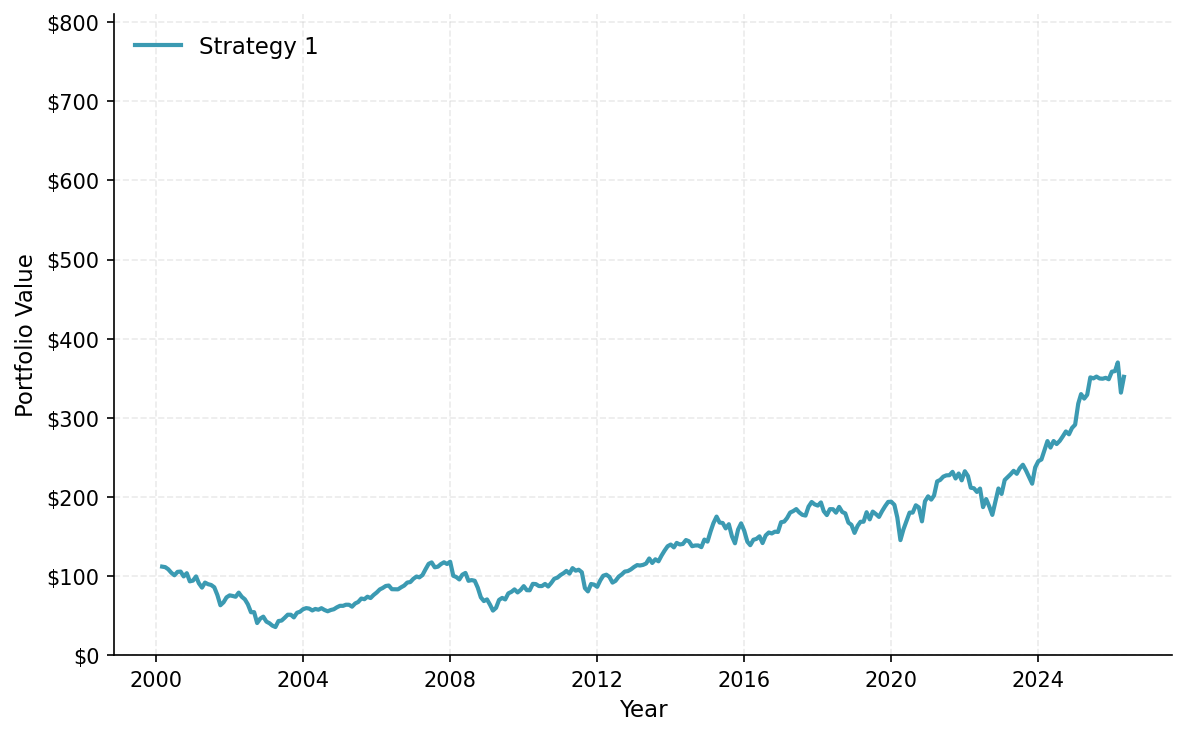
\includegraphics[width=\linewidth]{assets/GDAXI_strategy1.png}}%
            \only<2>{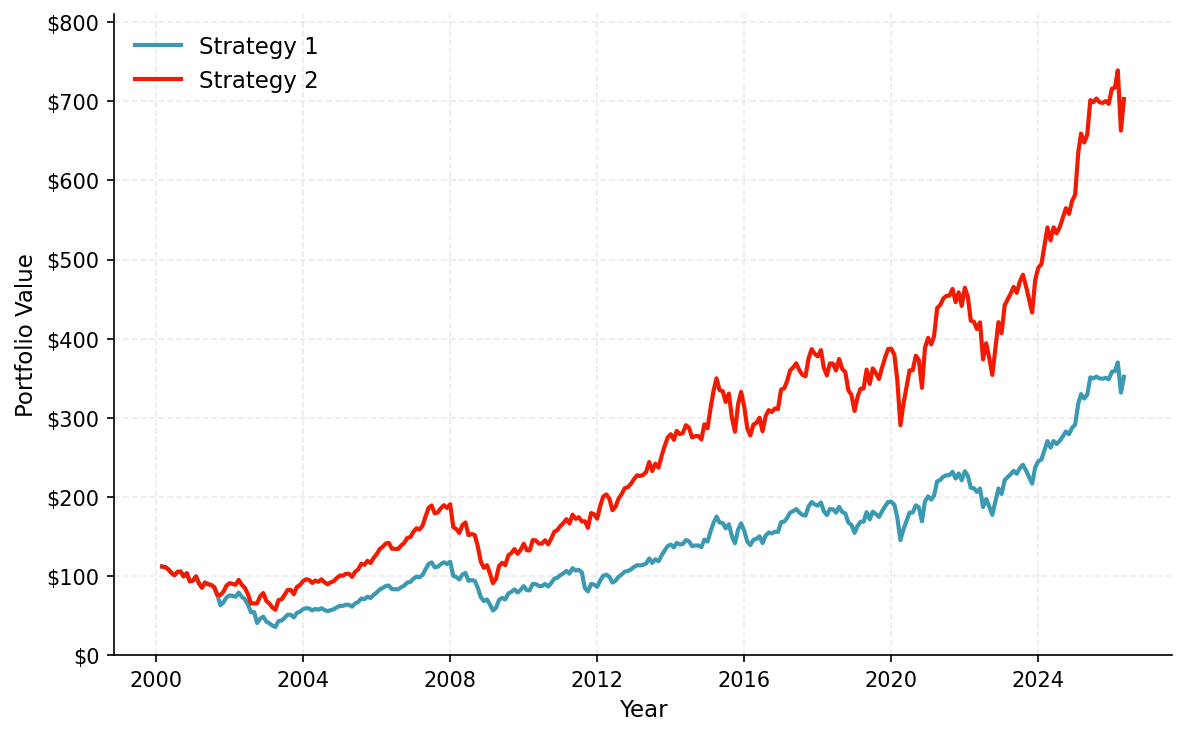
\includegraphics[width=\linewidth]{assets/GDAXI_linear.png}}%
            \only<3>{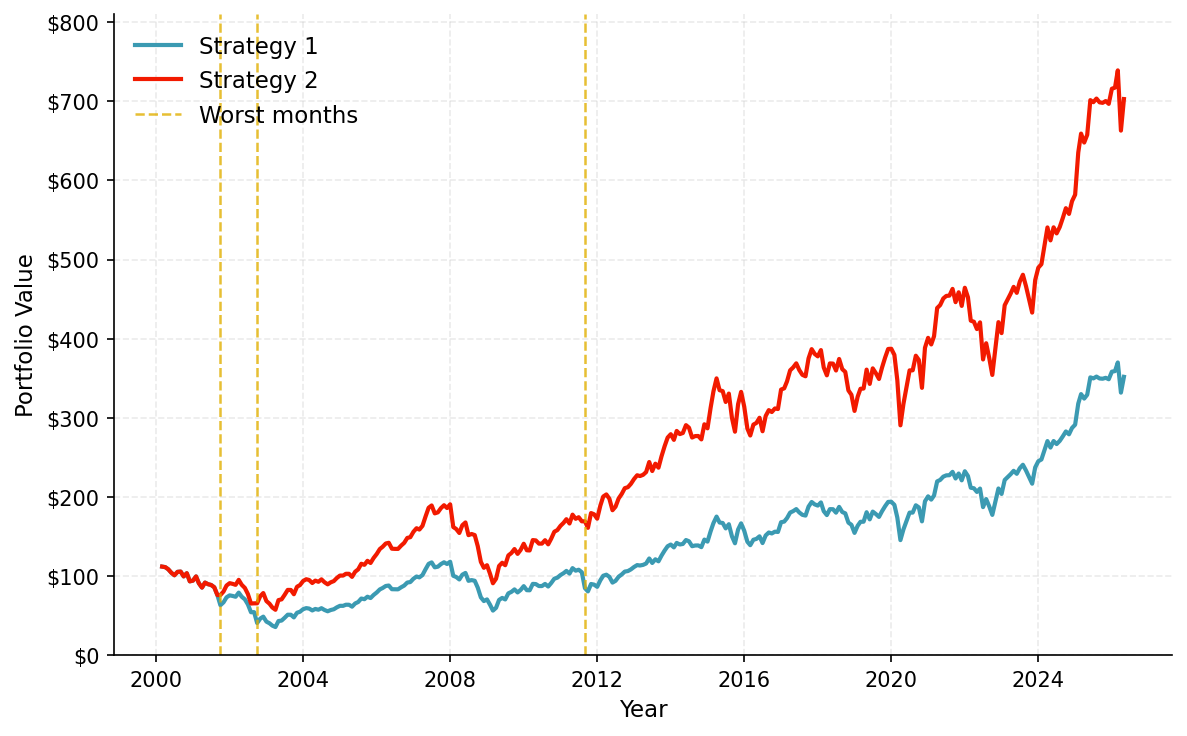
\includegraphics[width=\linewidth]{assets/GDAXI_worst_months.png}}%
            \only<4>{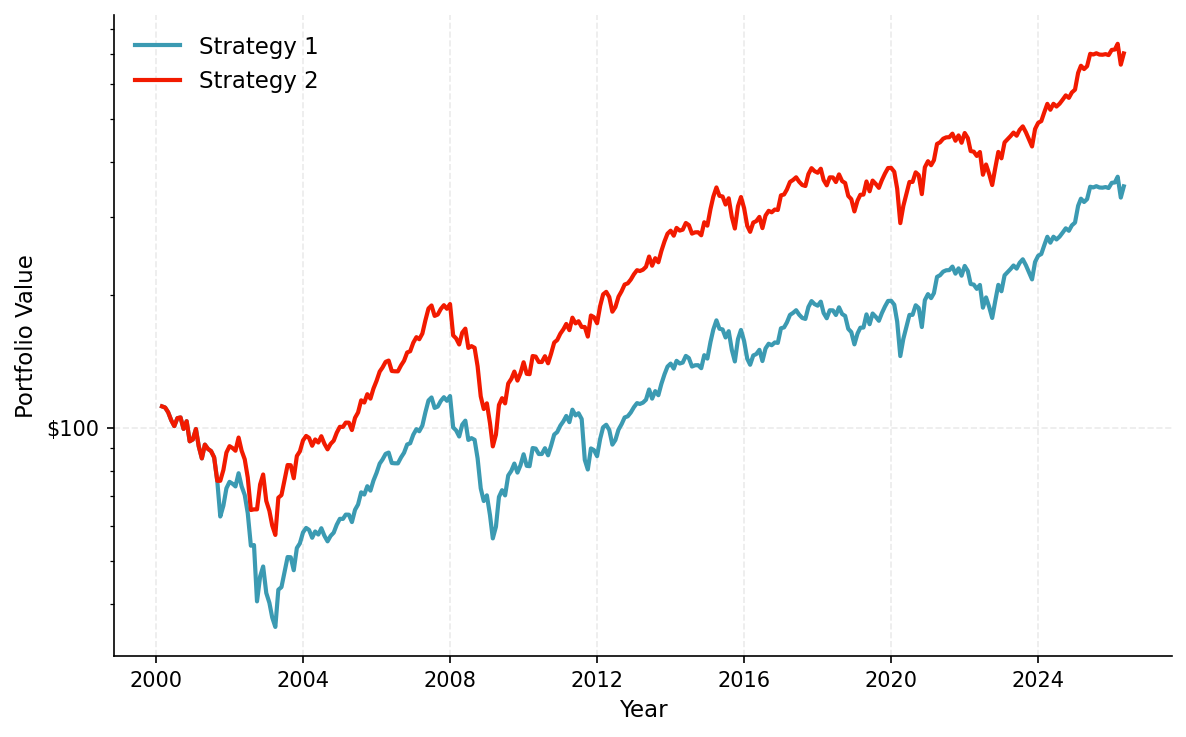
\includegraphics[width=\linewidth]{assets/GDAXI_log.png}}
        \end{figure}
    \end{frame}

    \begin{frame}{How Easy It Is to Fake Performance}
        \begin{itemize}\small
            \item \textbf{Strategy 2 = Strategy 1 minus the three worst months.}\\
            That's it. Delete three data points and the performance doubles.
            \vspace{0.8em}
            \item \textbf{The log scale tells the truth.} An investor entering at any later point would have experienced roughly the same returns from either strategy.
        \end{itemize}
        \pause
        \vfill
        \begin{rbox}{Three rows of data. One chart. A completely different conclusion.}
        No model was changed. No code was wrong. The only thing that changed was \textbf{which data was included} and that choice was (almost) invisible.
        \end{rbox}
    \end{frame}
    
\section{Tidy Finance}

    \begin{frame}{Tidy Finance is ...}
        \begin{itemize}
            \item ... an open-source project available at \href{https://www.tidy-finance.org}{www.tidy-finance.org} and published textbooks
            \item ... a step towards \textbf{reproducible finance} by providing a fully transparent code base
            \item ... a resource for students, lecturers, and professionals using \textbf{R} or \textbf{Python} for applications in finance
            \item ... a \textbf{tidy} approach to finance
            \item ... continuously maintained and expanded...
        \end{itemize}
    \end{frame}
    \begin{frame}{Tidy Finance is ...}
        \begin{figure}
            \centering
            \only<1>{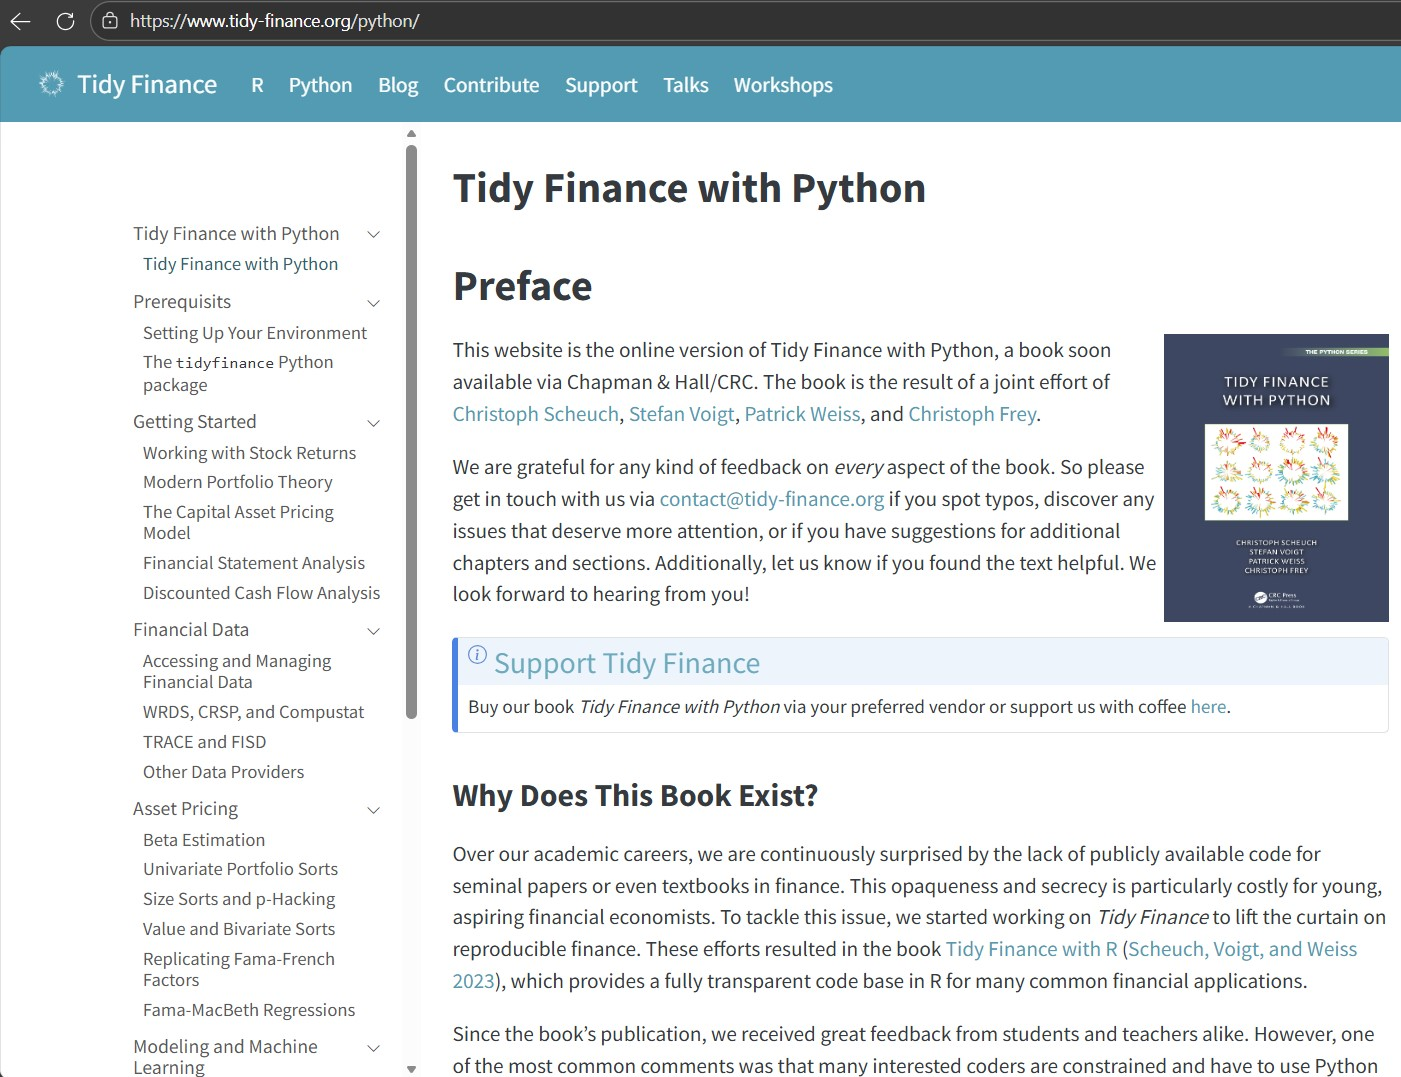
\includegraphics[width=0.8\linewidth]{assets/website3.jpg}}%
            \only<2>{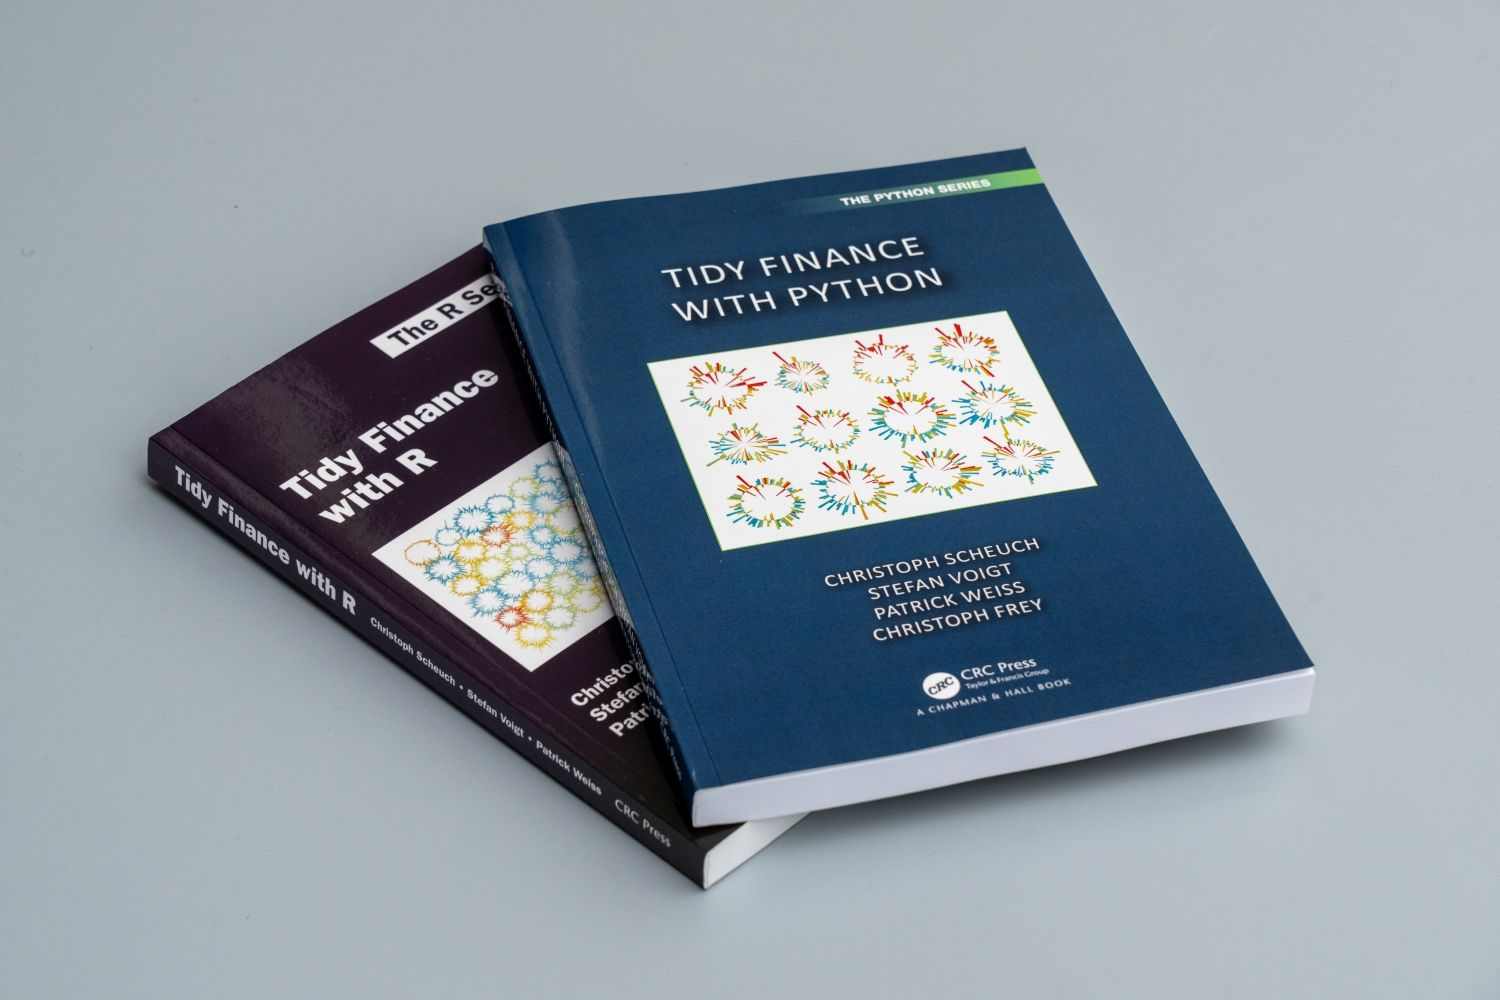
\includegraphics[width=0.8\linewidth]{assets/1724855421543.jpeg}}
        \end{figure}
    \end{frame}
    \begin{frame}{...Transparent}
        \begin{columns}[c]
            \begin{column}{0.2\textwidth}
                \only<1>{\textbf{Text}}     \only<2->{\textcolor{gray}{Text}}\\[6em]
                \only<2>{\textbf{Code}}     \only<1,3>{\textcolor{gray}{Code}}\\[6em]
                \only<3>{\textbf{Results}}  \only<1-2>{\textcolor{gray}{Results}}
            \end{column}
            \begin{column}{0.69\textwidth}
                \only<1>{\transparent{1}}\only<2->{\transparent{0.2}}%
                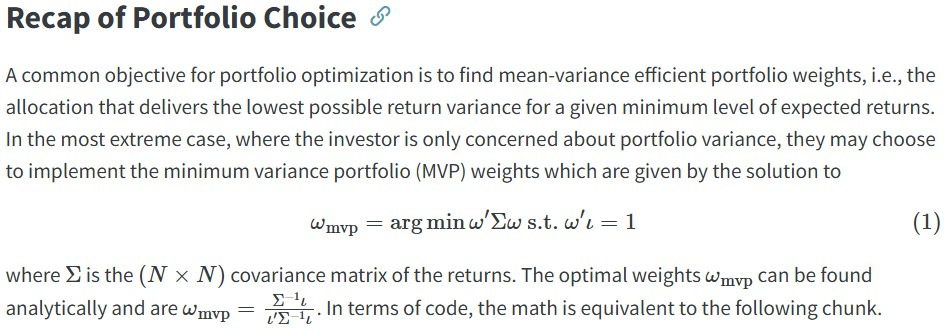
\includegraphics[width=\linewidth]{assets/text.jpg}\\[0.5em]
                \only<2>{\transparent{1}}\only<1,3>{\transparent{0.2}}%
                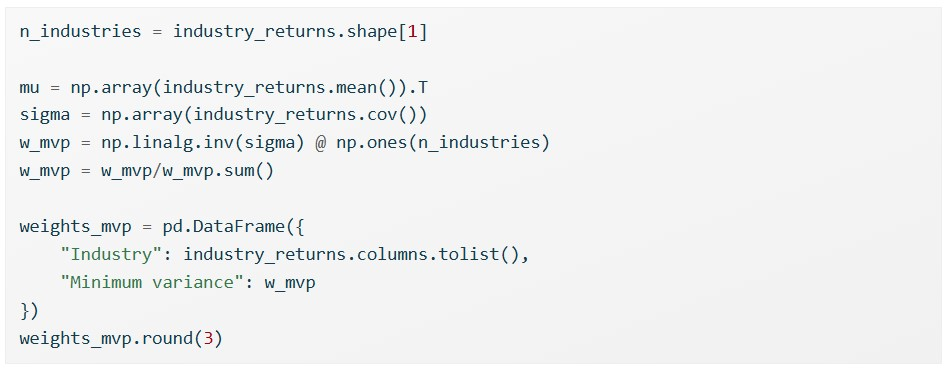
\includegraphics[width=\linewidth]{assets/code.jpg}\\[0.5em]
                \only<3>{\transparent{1}}\only<1-2>{\transparent{0.2}}%
                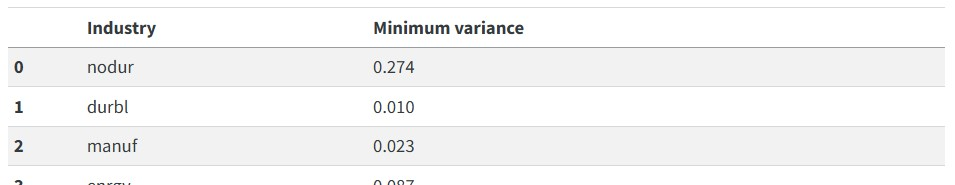
\includegraphics[width=\linewidth]{assets/results2.jpg}
            \end{column}
        \end{columns}
    \end{frame}

\section{The Tools}
\begin{frame}{Great Tools, One Side of the Story}
\begin{columns}[T]
\begin{column}{0.48\linewidth}
Python has excellent libraries for portfolio optimisation and backtesting.\\[0.5em]
\begin{itemize}\small
    \item \textbf{PyPortfolioOpt} --- mean-variance, Black-Litterman, risk parity in a few lines
    \item \textbf{backtesting.py} --- event-driven strategy backtests with built-in reporting
    \item \textbf{pyfolio / QuantStats} --- professional tear sheets and performance dashboards
\end{itemize}
\end{column}
\begin{column}{0.48\linewidth}
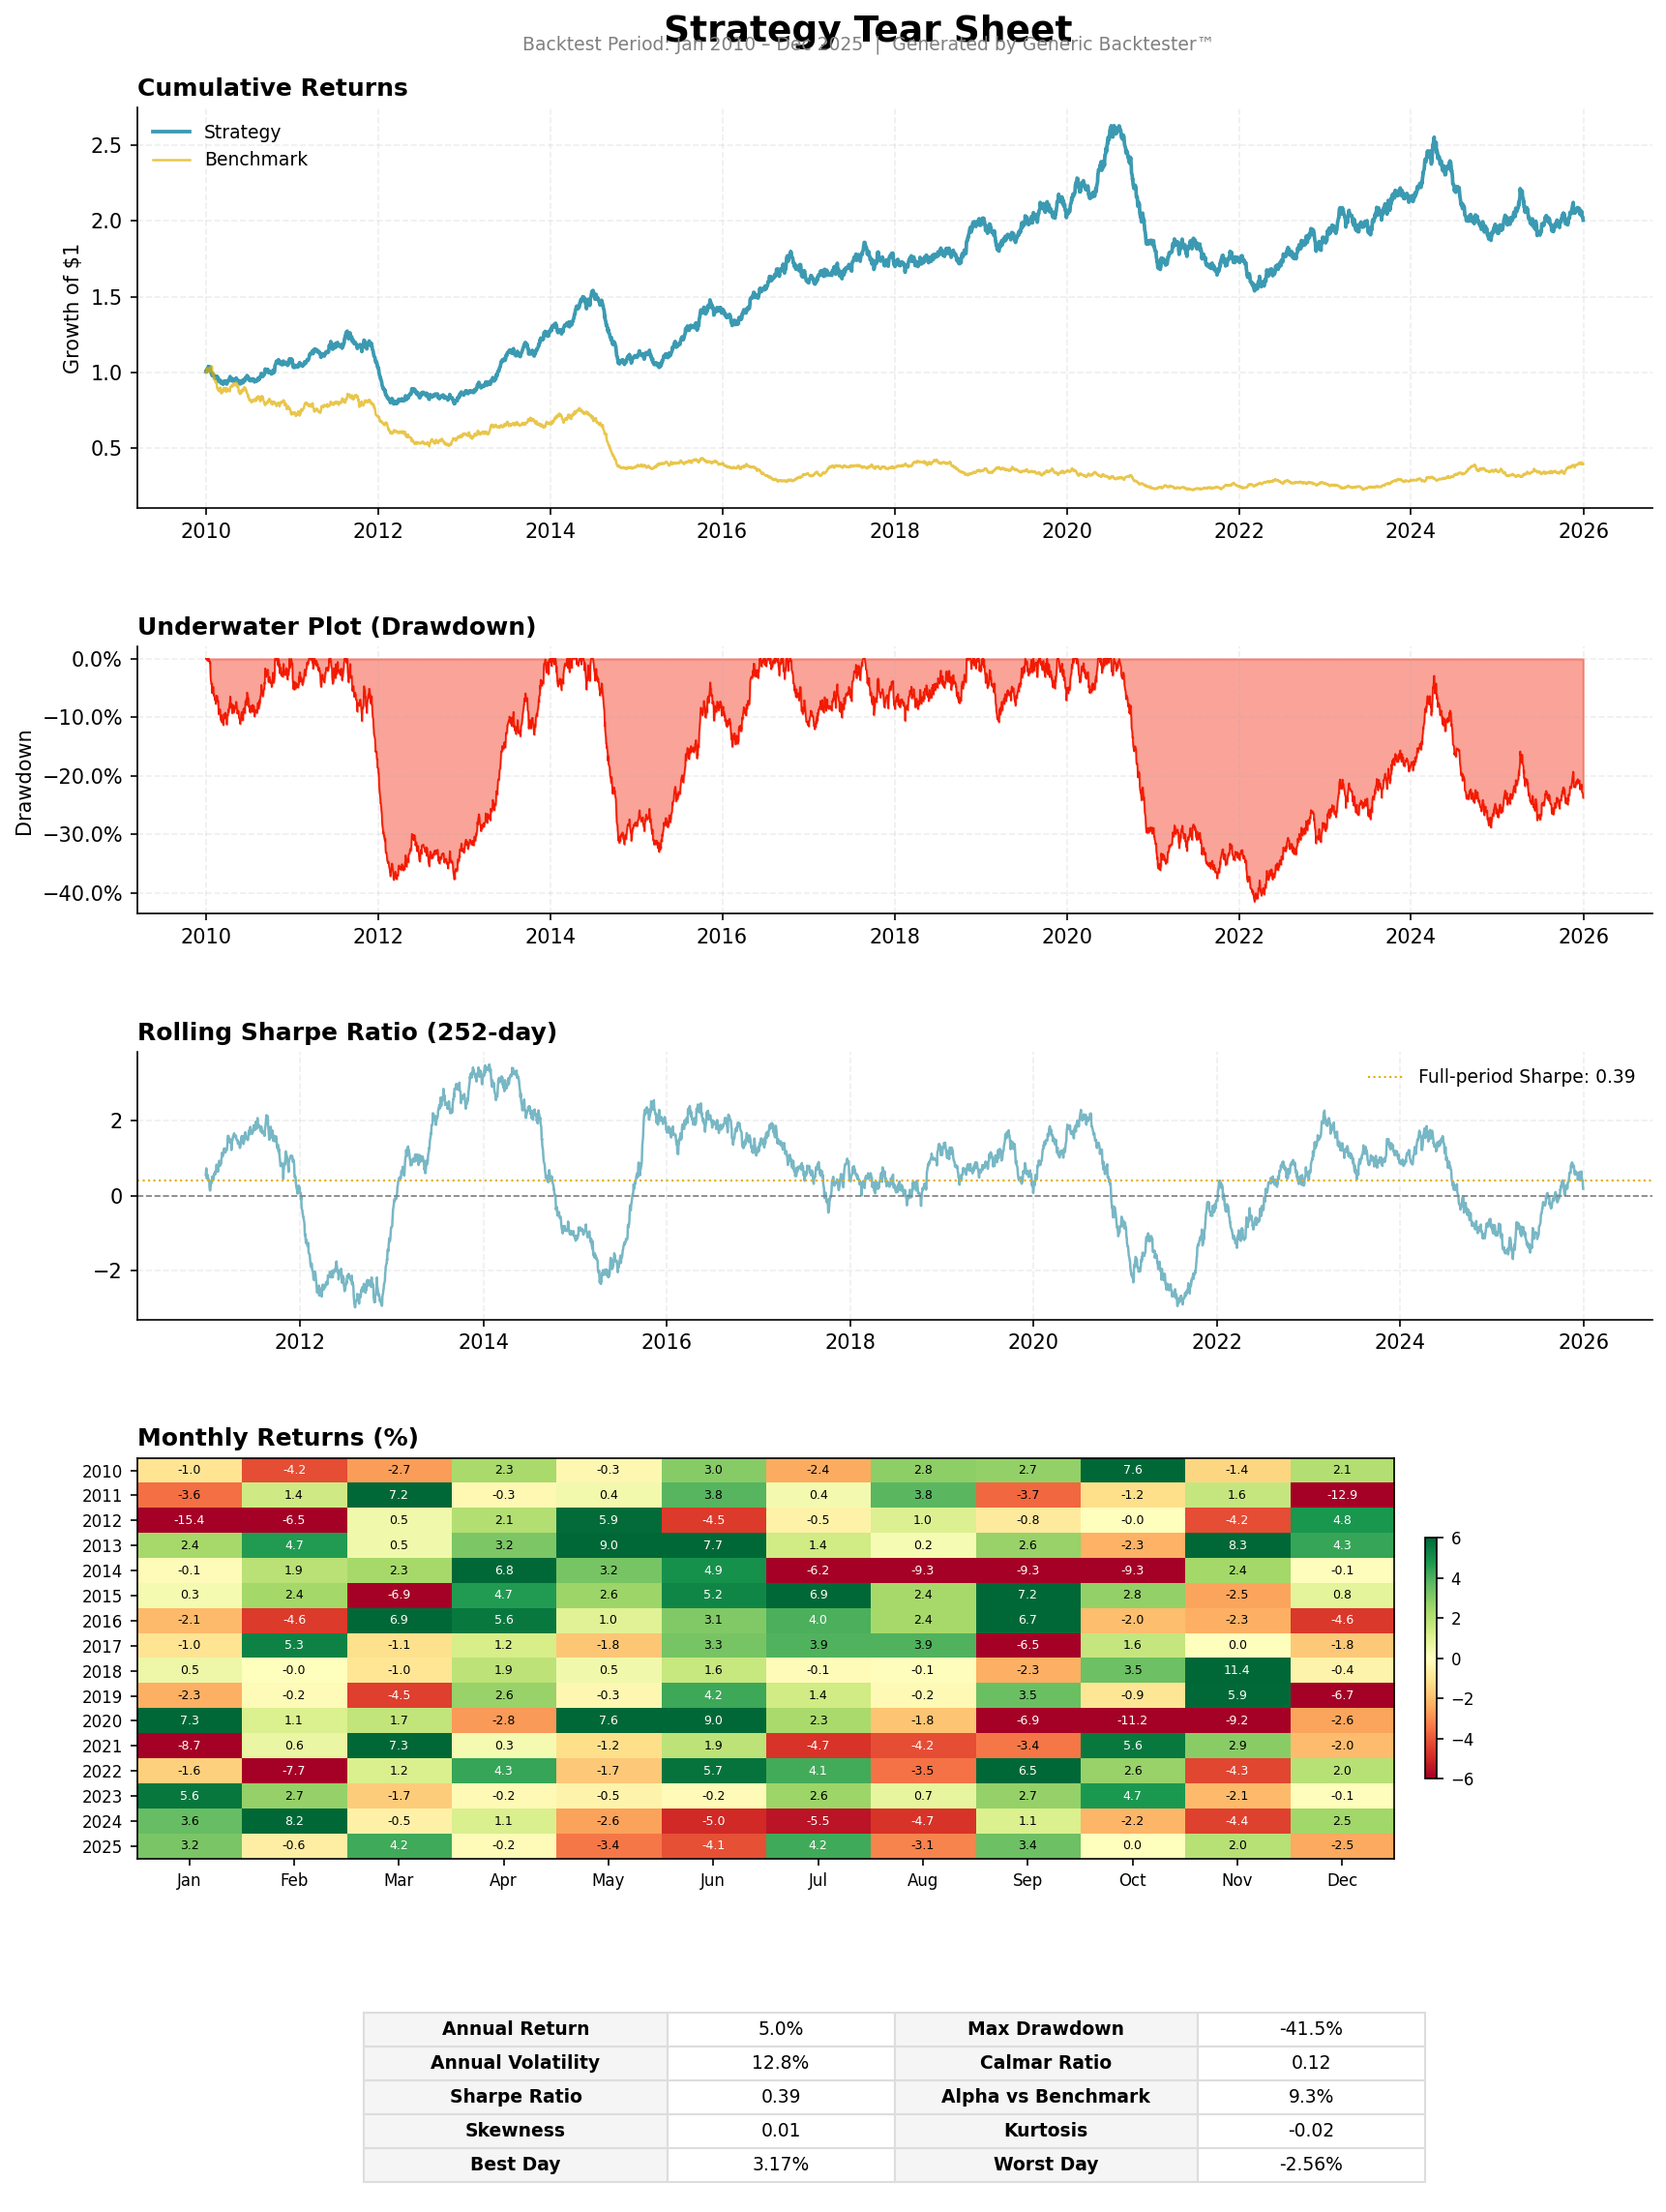
\includegraphics[width=\linewidth]{assets/tearsheet.png}
\end{column}
\end{columns}
\end{frame}
%=============================================================================
\begin{frame}{From Outputs to Inputs}
\begin{bbox}{They're good at what they do.}
These tools solve the \textbf{optimisation and evaluation} problem well.\\[0.3em]
But they start \emph{after} the critical decisions have been made: which data, which estimator, which costs, which sample.\\[0.3em]
The \textbf{input side} --- where the assumptions live --- is left entirely to you.
\end{bbox}
\end{frame}
%=============================================================================
\begin{frame}[plain]
\begin{center}
\vspace{2em}
{\Large\itshape ``Explicit is better than implicit.''}\\[1em]
{\normalsize PEP 20, \emph{The Zen of Python}}
\vspace{2em}
\end{center}
\end{frame}
%=============================================================================
\begin{frame}[fragile]{The One-Liner Optimizer}
\begin{lstlisting}
optimizer = PortfolioOptimizer(mu, S)
weights = optimizer.maximize_sharpe()
\end{lstlisting}
\small
\vspace{2em}
\begin{bbox}{Many defaults, typically hidden behind the scenes}
\begin{itemize}\footnotesize
    \item Which Return estimator? Arithmetic mean (not log, not CAPM)
    \pause
    \item Which Covariance matrix? Sample estimate with no shrinkage
    \pause
    \item Long-only constraint applied silently or long-short?
    \pause
    \item No transaction costs, no turnover constraints
\end{itemize}
\end{bbox}
\end{frame}

%=============================================================================
\begin{frame}[fragile]{Optimise First, Validate Later}
\begin{lstlisting}
# Try every combination, pick the best
for window in range(2, 101):
    for threshold in params:
        result = backtest(data, window, threshold)
        results.append(result)
 
best = max(results, key=lambda r: r.total_return)
 
# Then produce a professional dashboard
plot_performance(best.returns)
\end{lstlisting}
\vfill
\pause
\begin{rbox}{Two problems in one workflow}
\textbf{The sweep} is a hyperparameter search on the test set.\\[0.3em]
\textbf{The dashboard} validates the \emph{output}, not the \emph{process}. It takes whatever returns you give it and produces beautiful charts.
\end{rbox}
\end{frame}
%=============================================================================
\section{The Tidy Approach}
\begin{frame}{From Outputs to Inputs}
These libraries have made portfolio analysis accessible to everyone. They handle the hard parts well: optimisation, simulation, visualisation.\\[0.5em]
They are \textbf{designed} to take clean inputs and produce results. That's their job, and they do it well.\\[0.5em]
But every result depends on choices made \emph{before} you call the optimizer.
%\begin{itemize}\small
%    \item Is there survivorship bias in the data?
%    \item How are the input parameters estimated?
%    \item Is this in-sample or out-of-sample?
%\end{itemize}
\vfill
\pause
\begin{gbox}{This is where Tidy Finance comes in.}
To make the \textbf{input side} just as explicit, readable, and reproducible as the output side.
\end{gbox}
\end{frame}
%=============================================================================

%=============================================================================
\begin{frame}[fragile]{Every Assumption in Plain Sight}
From \emph{Tidy Finance} ``Constrained Optimization and Backtesting'':
\begin{lstlisting}
window_length = 120
beta = 50
gamma = 2

def evaluate_performance(w, w_prev, next_return, beta=50):
    raw_return = np.dot(next_return, w)
    turnover   = np.sum(np.abs(w - w_prev))
    net_return = raw_return - (beta/10000) * turnover
    return np.array([raw_return, turnover, net_return])
\end{lstlisting}
\vfill
\small
The cost model is right there.\\[0.5em]
The chapter applies the same approach to constraints: no short-selling, leverage limits, Regularization of the covariance matrix. Each one is an \textbf{explicit constraint} passed to \texttt{scipy.optimize.minimize}, not a silent default.
\end{frame}

\begin{frame}[fragile]{Every Assumption in Plain Sight: What We Optimize}
\begin{lstlisting}
def compute_efficient_weight_L1_TC(mu, sigma, gamma, beta, initial_weights):
    def objective(w):
        return (gamma * 0.5 * w.T @ sigma @ w - (1 + mu) @ w
            + (beta / 10000) / 2 * np.sum(np.abs(w - initial_weights)))
    # gradient(w): analytical derivative of objective
    constraints = {"type": "eq", "fun": equality_constraint,
        "jac": jacobian_equality}
    result = minimize(x0=initial_weights, fun=objective,
        jac=gradient, constraints=constraints,
        tol=options["tol"],  options={"maxiter": options["maxiter"]},
        method=options["method"])
    return result.x
\end{lstlisting}
\end{frame}

%=============================================================================
\begin{frame}[fragile]{Every Assumption in Plain Sight: One period at a time}
\begin{lstlisting}[escapechar=§]
for p in range(periods):
    returns_window = industry_returns.iloc[p:p+window_length§\marko{-1}§]
    next_return = industry_returns.iloc[p+window_length]
 
    sigma_window = np.array(returns_window.cov())
    mu = 0 * np.array(returns_window.mean())
 
    w_1 = compute_efficient_weight_L1_TC(
        mu, sigma_window, beta=50, gamma=2,
        initial_weights=w_prev_1)

    performance_values["MV (TC)"][p, :] = \
        evaluate_performance(w_1, w_prev_1, next_return)
\end{lstlisting}
\end{frame}

\begin{frame}{What Happens When You Forget the about the \texttt{-1}}
\begin{center}
    \only<1>{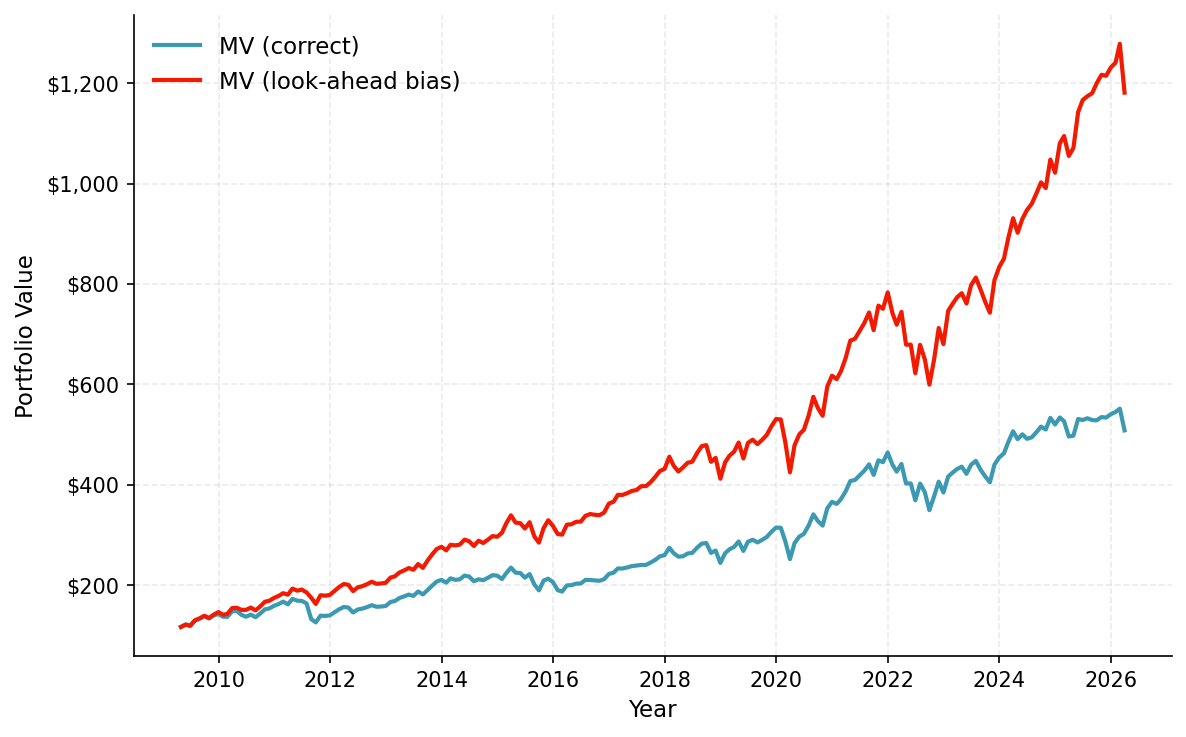
\includegraphics[width=\linewidth]{assets/markowitz_lookahead_bias.png}}%
    \only<2>{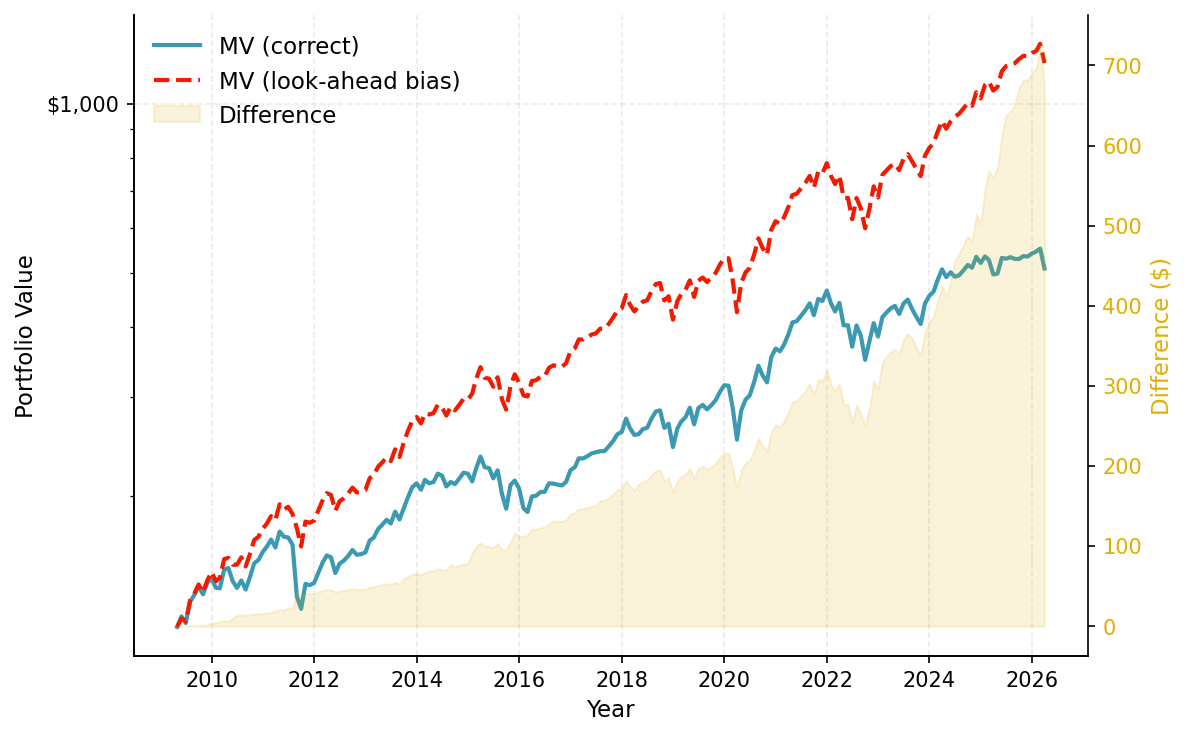
\includegraphics[width=\linewidth]{assets/markowitz_lookahead_bias_log.png}}
\end{center}
\vspace{-1em}
Forget the \texttt{-1} and you create the world famous \rtextb{look-ahead bias}
\end{frame}

\begin{frame}[fragile]{Infrastructure-as-Code for Backtesting}

\begin{gbox}{Infrastructure-as-Code for Backtesting}
Every assumption is a \textbf{visible line of R/Python code}.\\[0.3em]
As for infrastructure, it should be declared, versioned, and auditable.\\
\end{gbox}
\vspace{1em}
$\Rightarrow$ \textbf{Tidy Finance applies the same principle to empirical finance.}
\end{frame}

%=============================================================================
\begin{frame}{Same Principle, Every Chapter}

\begin{itemize}\small
    \item \textbf{CAPM \& Beta Estimation} \\ Which regression window? Which benchmark? Which frequency?
    \vspace{0.4em}
    \item \textbf{Fama-French Factor Replication} \\ Which breakpoints? Which weighting scheme? Which sample?
    \vspace{0.4em}
    \item \textbf{Option Pricing via Machine Learning} \\ Which features? Which train/test split? Which model complexity?
    \vspace{0.4em}
    \item \textbf{Financial Statement Analysis} \\ Which accounting variables? Which lag structure? Which universe?
\end{itemize}
\vfill
\begin{gbox}{One principle}
Every chapter, every topic: the assumptions are \textbf{explicit-by-default in the code}, not in your head.
\end{gbox}
\end{frame}
%=============================================================================
\section{Takeaway}
%=============================================================================
\begin{frame}{Three Things to Remember}
\begin{enumerate}\small
    \item \textbf{Explicit is better than implicit.}\\
    Not just for Python code style. For any analytical pipeline where the output drives decisions.
    \vspace{2em}
    \pause
    \item \textbf{If the assumption isn't in the code, it's in your head.}\\
    And that's where bad backtests, bad models, and bad data pipelines hide.
    \vspace{2em}
    \pause
    \item \textbf{Don't ask ``what's the Sharpe ratio?''}\\
    Ask ``what are your assumptions and where is your \gtextb{look-ahead bias}?''
\end{enumerate}
\end{frame}
%=============================================================================


\begin{frame}[plain]
\vspace*{2cm}
\begin{center}
{\Large\color{dblue}\url{https://www.tidy-finance.org}}\\[1.5em]
{\normalsize Open-source. Python \& R. Every assumption visible.}
\vspace{2em}
\end{center}
\end{frame}
\end{document}